
\section{Autoren}

Durch die im Abschnitt \ref{communities} gefundenen Communities kann man jetzt auch die Beziehung 
eines Autors zu der ihm zugeordneten Community betrachten. \\

% {Teilfrage: Sind verschieden Rollenverteilungen unter den Autoren einer Community erkennbar ?}
In diesem Abschnitt wird untersucht ob verschiedene Rollenverteilungen unter den Autoren einer Community erkennbar sind.
Falls verschiedene Rollenverteilungen auftreten, soll festgestellt werden, welche Rollen die Autoren einnehmen. Zus�tzlich k�nnten die Rollen der Autoren, welche am 
meisten publizieren, betrachtet werden. \\

% { Methoden }

Um die Autoren mit verschiedenen Rollen charakterisieren zu k�nnen, werden die in \cite{hubsconnectors} beschriebene Klassifizierung von Knoten verwendet. F�r diese Klassifizierung muss f�r jeden Knoten der \textit{Within-module degree} (z-score) und der \textit{Participation coefficient} berechnet werden. 

\subsection{Metriken eines Autors}

In Abbildung \ref{fig:r1_r7} ist nun die Klassifizierung der Knoten zu erkennen.


\begin{center}
					\hpic{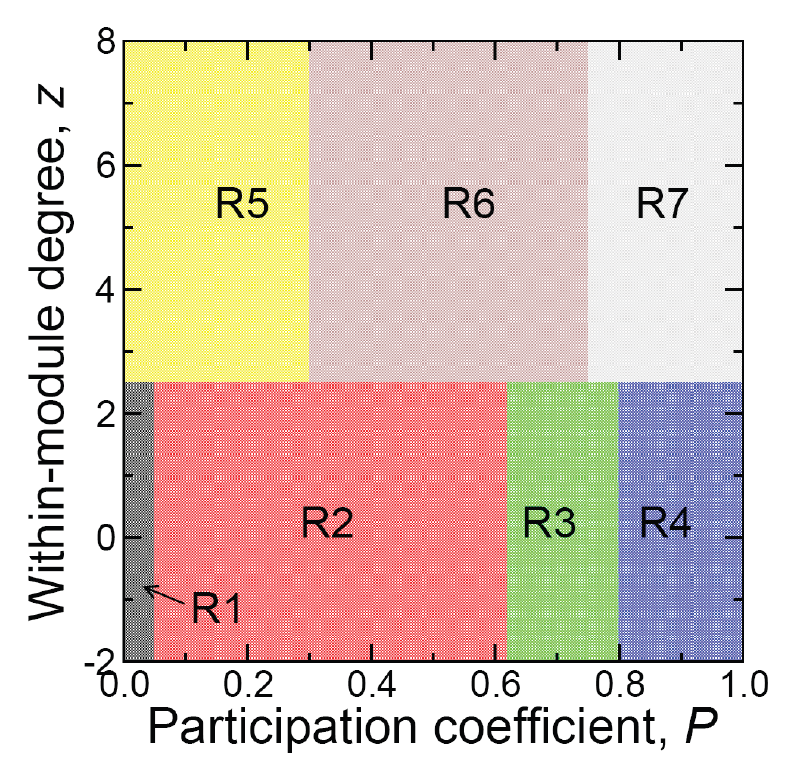
\includegraphics[width=0.7\textwidth]{images/r1_r7.png}
					} \newcaption{Klassifizierung der Author-Knoten }
					\label{fig:r1_r7}
					(Quelle: \cite{hubsconnectors})
\end{center}

In diesem Modell wird zwischen folgenden Rollen unterschieden (Es wurde versucht, eine m�glichst passende deutsche �bersetzung zu finden ):

\begin{itemize}

\item Nabenknoten (hubs) 

\begin{description}
 \item [(R5) provincial hubs] (provinzielle Naben/Zentren)
 \item [(R6) connector hubs] (verbindende Naben/Zentren)
 \item [(R7) kinless hubs] (sippenlose Naben/Zentren)
\end{description}

 \item Einzelknoten (non-hubs) 
\begin{description}
 \item [(R1) ultraperipheral] (sehr dezentral)
 \item [(R2) peripheral] (dezentral)
 \item [(R3) connectors] (Bindeglieder)
 \item [(R4) kinless vertices] (Einzelknoten)
\end{description}

\end{itemize}

Zur Klassifizierung der Autor-Knoten im Co-Autor-Graphen, wird f�r jeden Knoten die Community betrachtet in der er sich befindet (Top-Level-Community). 

\subsubsection{Within-module degree}


Der Within-module degree eines Autors ist durch folgende Formel \cite[p.84]{conductance} bestimmt: \\

\begin{center}
\hpic{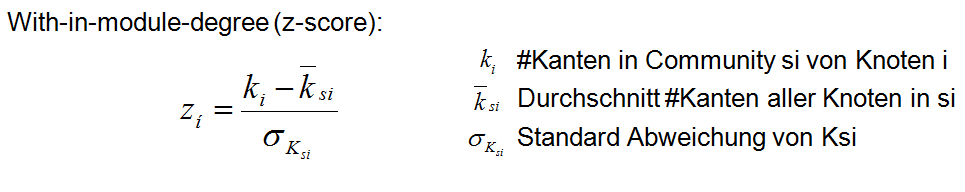
\includegraphics[width=0.7\textwidth]{images/with_in_module}
					} \newcaption{Formel zur Berechnung des Within-module degree}
					\label{form:Within-module-form  }
					Quelle:(\cite{conductance})
\end{center}


\subsubsection{Participation coefficient}

Der Participation coefficient eines Autors ist durch folgende Formel \cite[p.84]{conductance} bestimmt: \\

\begin{center}
\hpic{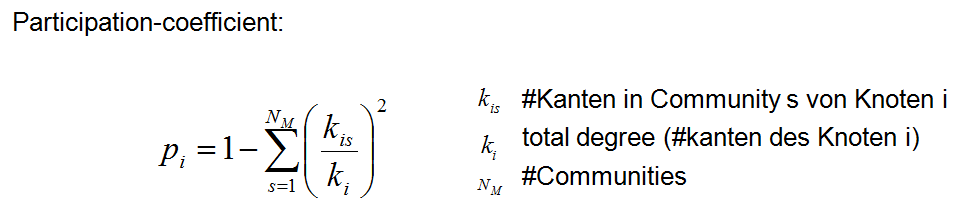
\includegraphics[width=0.7\textwidth]{images/part_coeff}
					} \newcaption{Formel zur Berechnung des Participation coefficient}
					\label{form:Participation-coefficient-form  }
					Quelle:(\cite{conductance})

\end{center}

% { Ergebnisse }


\subsection{Ergebnisse der Messungen}

In Abbildung \ref{fig:hub_con_dist} ist die Verteilung zwischen \textit{Hubs} und \textit{Connectors} zu erkennen. Die Anzahl der Autoren ist dabei in Tausend angegeben. 

\begin{center}
					\hpic{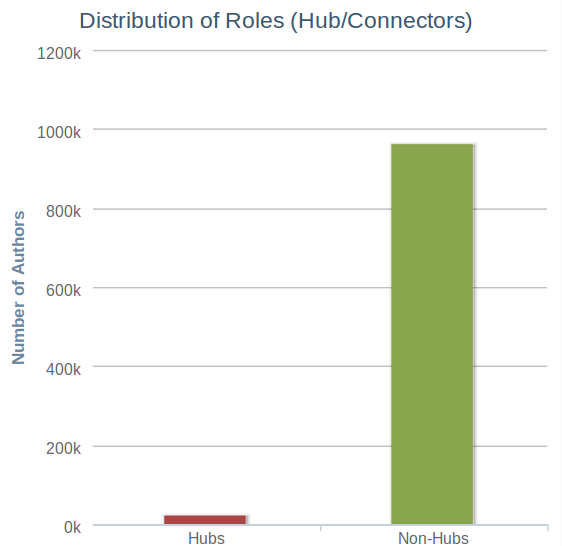
\includegraphics[width=0.7\textwidth]{results/roles_hub_con}
					} \newcaption{Verteilung der Rollen hubs/connectors}
					\label{fig:hub_con_dist}
\end{center}

Abbildung \ref{fig:r1_r7_dist} zeigt nun die Verteilung auf alle Rollen. Es wurden zu jeder definierten Rolle Autoren gefunden. Dabei gibt es am Meisten \textit{R1 Autoren} und am wenigsten \textit{R7 Autoren}.


\begin{center}
					\hpic{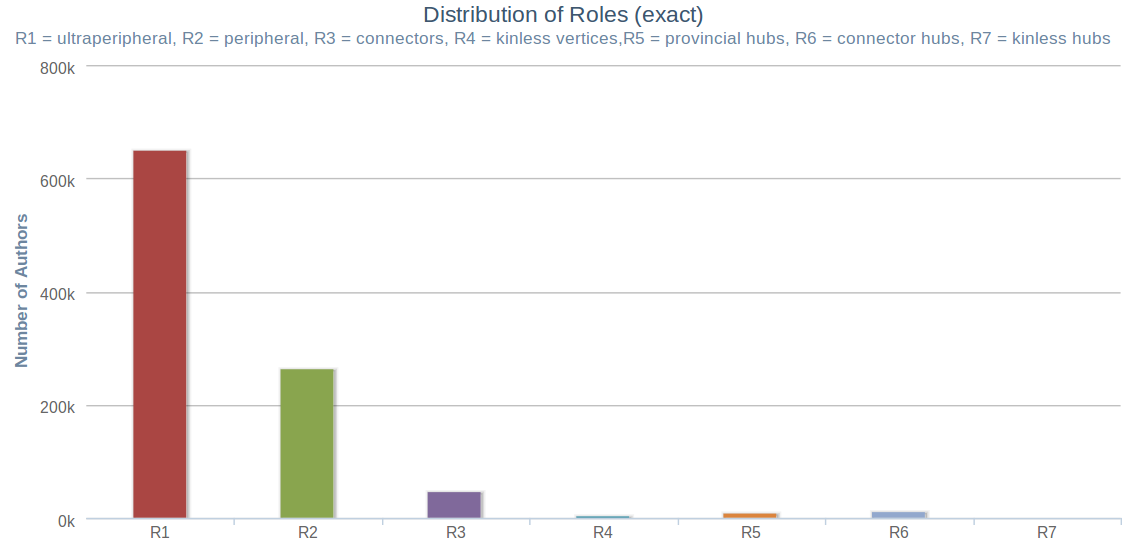
\includegraphics[height=0.7\textwidth,angle=90]{results/roles_r1r7}
					} \newcaption{Verteilung der Rollen R1-R7}
					\label{fig:r1_r7_dist}
\end{center}

\subsection{Meist publizierende Autoren}

Folgende Tabelle zeigt verschiedene Details der meist publizierenden Autoren (Top 16 der DBLP - Stand 26.01.2012). Dabei beziehen sich die Conductance und die Gr��e auf die Community in der sich der Autor befindet.

\begin{table}
    \begin{tabular}{|l|l|l|l|l|}
        \hline
        \textbf{Name }    & \textbf{Anzahl Publikationen} &\textbf{ Rolle} & \textbf{Conductance}   & \textbf{Gr��e }    \\ \hline 
        Philip S. Yu      & 657                  & R7    & 1,041                         & 18693                    \\ \hline
        Chin-Chen Chang   & 653                  & R6    & 0,291                         & 26008                    \\ \hline
        Elisa Bertino     & 624                  & R7    & 0,946                         & 19384                    \\ \hline
        Thomas S. Huang   & 620                  & R6    & 0,563                         & 83723                    \\ \hline
        Wen Gao           & 617                  & R5    & 0,563                         & 83723                    \\ \hline
        Ming Li           & 589                  & R6    & 0,563                         & 83723                    \\ \hline
        Jun Wang          & 583                  & R6    & 0,563                         & 83723                    \\ \hline
        H. Vincent Poor   & 574                  & R6    & 0,768                         & 19267                    \\ \hline
        Edwin R. Hancock  & 548                  & R6    & 0,716                         & 796                      \\ \hline
        Wei Wang          & 533                  & R6    & 0,563                         & 83723                    \\ \hline
        Mario Piattini    & 532                  & R6    & 0,755                         & 18781                    \\ \hline
        Jiawei Han        & 531                  & R6    & 0,563                         & 83723                    \\ \hline
        Sudhakar M. Reddy & 525                  & R6    & 0,643                         & 18789                    \\ \hline
        Yan Zhang         & 524                  & R6    & 0,563                         & 83723                    \\ \hline
        Wei Liu           & 497                  & R6    & 0,563                         & 83723                    \\ \hline
        Hans-Peter Seidel & 494                  & R6    & 0,756                         & 17123                    \\
        \hline
    \end{tabular}
\end{table}


\subsection{ Analyse der Messergebnisse }

Es kann eine Rollenverteilung im Co-Autor-Graphen erkannt werden, wobei die meisten Autoren die \textit{(R1) ultraperipheral Rolle} einnehmen. Die meist publizierenden Autoren, welche n�her betrachtet wurden, nehmen alle eine \textit{Hub Rolle} ein. Auch sind diese Autoren in Communities mit recht hohen Conductance Werten. Dies bedeutet, dass diese Communities stark mit anderen Communities verbunden sind. Einige der meist publizierenden Autoren sind in der gr��ten Community.

% { Diskussion }


